\documentclass[a4paper,12pt]{article}

\usepackage{mystyle}
\usepackage{gensymb}


\usepackage{scalerel}
\usepackage{stackengine}

\graphicspath{ {images/} }


% https://tex.stackexchange.com/questions/5461/is-it-possible-to-change-the-size-of-an-arrowhead-in-tikz-pgf
\usetikzlibrary{arrows.meta}


\DeclareMathOperator{\Image}{Im}

\definecolor{pink}{RGB}{218, 3, 174}
\definecolor{violet}{RGB}{148, 0, 211}
\definecolor{green}{RGB}{0, 153, 0}
\definecolor{orange}{RGB}{255, 153, 0}
\definecolor{blue}{RGB}{5, 73, 255}


% https://tex.stackexchange.com/a/101138/135045

\newcommand\widesim[1]{\ThisStyle{%
  \setbox0=\hbox{$\SavedStyle#1$}%
  \stackengine{-.1\LMpt}{$\SavedStyle#1$}{%
    \stretchto{\scaleto{\SavedStyle\mkern.2mu\sim}{.5150\wd0}}{.6\ht0}%
  }{O}{c}{F}{T}{S}%
}}

\newcommand{\BigMiddleThree}{\;\left|\vphantom{\begin{pmatrix} 0\\0\\0 \end{pmatrix}}\right.\;}
\newcommand{\BigMiddleFour}{\;\left|\vphantom{\begin{pmatrix} 0\\0\\0\\0 \end{pmatrix}}\right.\;}


% https://tex.stackexchange.com/questions/63531/how-to-write-quotation-marks-in-math-environment
\DeclareMathSymbol{\mlq}{\mathord}{operators}{``}
\DeclareMathSymbol{\mrq}{\mathord}{operators}{`'}


\DeclareMathOperator{\Imag}{Im}


% https://tex.stackexchange.com/questions/544453/undefined-control-sequence-after-paragraph
\renewcommand{\paragraph}[1]{\noindent\textbf{#1}\quad}


% https://tex.stackexchange.com/questions/36851/skipping-line-after-proof-in-proof-environment#comment73553_36851
\newcommand{\proofindent}{\hspace*{\fill}\par\vspace{0.5em}\noindent}

% https://tex.stackexchange.com/questions/63531/how-to-write-quotation-marks-in-math-environment
\DeclareMathSymbol{\mlq}{\mathord}{operators}{``}
\DeclareMathSymbol{\mrq}{\mathord}{operators}{`'}


% https://tex.stackexchange.com/questions/210290/how-to-write-doubleprime-in-latex
\newcommand*{\dprime}{{\prime\prime}\mkern-1.2mu}



\author{Алексеев Василий}


\title{Семинар 9}
\date{7 + 11 апреля 2023}


\begin{document}
  \maketitle
  
  \tableofcontents

  \thispagestyle{empty}
  
  \newpage
  
  \pagenumbering{arabic}


  \section{Bili \& Qua (Diag 2)}
  
  \emph{
    В конспекте билинейная функция называется именно ``билинейной функцией''.
    Хотя общепринятым синонимом является также термин ``билинейная форма''.
    Квадратичная функция же иногда в конспекте именуется и ``квадратичной формой'' (общепринятый синоним), и даже просто ``формой'' (немного неряшливое короткое обозначение, которое, однако, можно считать корректным, но только в рамках конспекта~---~неопределённости возникнуть не должно, потому что билинейная функция ``формой'' именоваться не будет).
  }
  
  \subsection{Билинейная b(x, y) и квадратичная k(x) функции}
  
  Линейное отображение $\phi\colon X \hm\to \RR$ называлось \emph{линейной функцией}.
  То есть линейная функция принимает \emph{один} вектор, и возвращает число.
  Но отображения вообще могут принимать на вход и \emph{больше одного} аргумента.
  (Например, хотя бы та же операция сложения векторов $\mlq{+}\mrq\colon X \hm\times X \hm\to X$.)
  Рассматривая функции \emph{от двух} аргументов, можно бы было выделить класс функций, линейных только по первому аргументу, только по второму или \emph{по двум аргументам сразу}.
  Приходим к следующему понятию.
  
  \begin{definition}
    \emph{Билинейной функцией} называется отображение $b\colon X \hm\times X \hm\to \RR$, линейное по каждому аргументу:
    \[
      \left\{
        \begin{aligned}
          &b(\bds x_1 + \bds x_2, \bds y) = b(\bds x_1, \bds y) + b(\bds x_2, \bds y)\\
          &b(\alpha \bds x, \bds y) = \alpha b(\bds x, \bds y)
        \end{aligned}
      \right.
      \quad \left\{
        \begin{aligned}
          &b(\bds x, \bds y_1 + \bds y_2) = b(\bds x, \bds y_1) + b(\bds x, \bds y_2)\\
          &b(\bds x, \beta \bds y) = \beta b(\bds x, \bds y)
        \end{aligned}
      \right.
    \]
  \end{definition}
  
  Отдельно стоит выделить билинейные функции, значения которых не зависят от порядка аргументов.
  
  \begin{definition}
    Билинейная функция $b(\cdot, \cdot)$ называется \emph{симметричной}, если
    \[
      b(\bds x, \bds y) = b(\bds y, \bds x),\quad \forall \bds x, \bds y \in X
    \]
  \end{definition}
  
  \begin{example}
    Симметричная билинейная функция~---~это, например, скалярное произведение векторов геометрического векторного пространства:
    \begin{equation}\label{eq:bili-example}
      b(\bds x, \bds y) = (\bds x, \bds y) = |\bds x| |\bds y| \cos\angle(\bds x, \bds y)
    \end{equation}
  \end{example}
  
  От линейной функции (один аргумент) перешли к билинейной функции (два аргумента).
  А что, если...
  в качестве обоих аргументов в билинейную функцию подать один и тот же вектор?
  Снова получится функция одного аргумента.
  
  \begin{definition}
    Пусть $b(\cdot, \cdot)$~---~симметричная билинейная функция\footnote{
      Как могло бы сперва показаться, дело не в том, что если $b(\cdot, \cdot)$ не симметричная, то $k(\cdot)$ всегда ноль.
      Нет.
      Например, $b(\bds x, \bds y) \hm= -2 x_1 y_2$ не симметричная (это формула билинейной функции от координат векторов~---~про этот способ описания билинейной функции будет далее в конспекте).
      И \emph{можно} было бы подставить вместо вектора $\bds y$ тоже вектор $\bds x$ и получить $b(\bds x, \bds x) \hm= -2 x_1 x_2$.
      Но тогда по формуле квадратичной функции, если не знать, что $b(\cdot, \cdot)$ была симметричной, нельзя однозначно восстановить матрицу этой билинейной функции (будет несколько возможных вариантов).
      Вообще, матрицу любой билинейной функции можно представить как сумму симметричной и кососимметричной матриц (см.~\# 15.94).
      Можно показать, что, кососимметричная вообще не будет играть роли в формуле квадратичной функции, порождаемой данной билинейной.
      (Например, ту же $b(\bds x, \bds y) \hm= -2 x_1 y_2$ можно так представить как сумму симметричной и кососимметричной частей: $-2 x_1 y_2 \hm= (-x_1 y_2 \hm- x_2 y_1) \hm+ (-x_1 y_2 \hm+ x_2 y_1)$.
      Несложно проверить, что при вычислении $k(\bds x) \hm= b(\bds x, \bds x)$ кососимметричная часть занулится.)
      То есть если по произвольной билинейной функции как бы ``построить'' квадратичную, положив $k(\bds x) \hm= b(\bds x, \bds x)$, то эта квадратичная по сути будет определяться только ``симметричной частью'' билинейной функции...
      В общем, с ``симметричной'' в определении квадратичной функции получается более однозначно)
    }.  % https://math.stackexchange.com/questions/1158912/why-is-quadratic-form-defined-via-a-symmetric-bilinear-form
    Тогда \emph{квадратичной функцией}, порождённой $b(\cdot, \cdot)$, называется отображение $k\colon X \hm\to \RR$, которое определяется формулой:
    \[
      k(\bds x) = b(\bds x, \bds x)
    \]
  \end{definition}
  
  \begin{example}
    Симметричной билинейной функцией~(\ref{eq:bili-example}) порождается следующая квадратичная:
    \begin{equation}\label{eq:qua-example}
      k(\bds x) = b(\bds x, \bds x) = (\bds x, \bds x) = |\bds x|^2
    \end{equation}
  \end{example}
  
  Будет ли квадратичная функция линейной?
  Очевидно, функция из примера~(\ref{eq:qua-example}) линейной вообще не будет.
  Посмотрим, чему будет равен образ суммы $\bds x_1 \hm+ \bds x_2$ под действием произвольной квадратичной функции~$k(\cdot)$:
  \[
    \underline{k(\bds x_1 + \bds x_2)}
    = b(\bds x_1 + \bds x_2, \bds x_1 + \bds x_2)
    = b(\bds x_1, \bds x_1) + b(\bds x_2, \bds x_2) + b(\bds x_1, \bds x_2) + b(\bds x_2, \bds x_1)
    = \underline{k(\bds x_1) + k(\bds x_2) + 2 b(\bds x_1, \bds x_2)}
  \]
  то есть тоже в общем случае не линейная.
  Из формулы выше также можно заметить следующее.
  Значение билинейной функции $b(\cdot, \cdot)$ на произвольной паре векторов $\bds x_1, \bds x_2$ можно выразить с помощью соответствующей ей квадратичной функции:
  \[
    \boxed{
      b(\bds x_1, \bds x_2) = \frac{k(\bds x_1 + \bds x_2) - k(\bds x_1) - k(\bds x_2)}{2}
    }
  \]
  то есть, с одной стороны, квадратичная порождается симметричной билинейной, и, с другой~---~по квадратичной однозначно восстанавливается породившая её симметричная билинейная~(\ref{fig:vector-scalar}).
  
  \begin{figure}[h!]
    \centering
  
    \includegraphics[width=0.5\columnwidth]{vector-scalar}
  
    \caption{Можно вычислить скалярное $(\bds a, \bds b)$, зная длины $|\bds a|$, $|\bds b|$ и $|\bds a \hm+ \bds b|$.}
    \label{fig:vector-scalar}
  \end{figure}
  
  Из всех квадратичных функций на пространстве~$X$ выделяют несколько классов.
  
  \begin{definition}
    Квадратичная функция~$k(\cdot)$ называется
    \begin{itemize}
      \item \emph{положительно определённой}, если $k(\bds x) \hm> 0$, $\bds x \hm{\not=} \bds 0$,
      \item \emph{отрицательно определённой}, если $k(\bds x) \hm< 0$, $\bds x \hm{\not=} \bds 0$,
      \item \emph{положительно полуопределённой}, если $k(\bds x) \hm\geq 0$, $\forall \bds x$,
      \item \emph{отрицательно полуопределённой}, если $k(\bds x) \hm\leq 0$, $\forall \bds x$.
    \end{itemize}
  \end{definition}
  
  \begin{example}
    Если рассматривать множество векторов~--~направленных отрезков трёхмерного пространства, то форма $k(\bds x) \hm= |\bds x|^2$~(\ref{eq:qua-example}) будет положительно определённой.
    Форма же $k(\bds x) \hm= -|\bds x|^2$ будет отрицательно определённой.
    Пример же полуопределённой формы... на данном этапе привести затруднительно.
    ...Или нет.
    Да, например, пусть $\bds a \hm{\not=} \bds 0$.
    Тогда определим форму следующим образом:
    \[
      k(\bds x) = \left|\frac{(\bds x, \bds a)}{|\bds a|^2} \bds a\right|^2
    \]
    то есть как квадрат ортогональной проекции вектора~$\bds x$ на направление, задаваемое вектором~$\bds a$ (это в самом деле квадратичная форма, так как она порождена симметричной билинейной функцией $b(\bds x, \bds y)$, которая по паре векторов $\bds x, \bds y$ возвращает скалярное произведение их ортогональных векторных проекций на $\bds a$).
    Очевидно, $k(\bds x) \hm\geq 0$ для любого~$\bds x$.
    Однако $k(\bds x)$ может быть равна нулю и при $\bds x \hm{\not=} \bds 0$ (если $\bds x \hm\perp \bds a$). 
  \end{example}
  
  
  \subsection{Матрица b(x, y)}
  
  \begin{example}
    Пусть в трёхмерном геометрическом пространстве векторов введён базис $e \hm= (\bds e_1, \bds e_2, \bds e_3)$.
    Распишем формулу для скалярного произведения произвольной пары векторов $\bds x$ и $\bds y$, разложив каждый из них по базису~$e$:
    \begin{equation*}
    \begin{split}
      (\bds x, \bds y)
      &= (x_1 \bds e_1 + x_2 \bds e_2 + x_3 \bds e_3, y_1 \bds e_1 + y_2 \bds e_2 + y_3 \bds e_3)\\
      &= x_1 (\bds e_1, \bds e_1) y_1 + x_1 (\bds e_1, \bds e_2) y_2 + x_1 (\bds e_1, \bds e_3) y_3 +\\
      &\hphantom{= {}}\; x_2 (\bds e_2, \bds e_1) y_1 + x_2 (\bds e_2, \bds e_2) y_2 + x_2 (\bds e_2, \bds e_3) y_3 +\\  % TODO: need "reliable" spacing
      &\hphantom{= {}}\; x_3 (\bds e_3, \bds e_1) y_1 + x_3 (\bds e_3, \bds e_2) y_2 + x_3 (\bds e_3, \bds e_3) y_3
    \end{split}
    \end{equation*}
    
    ``Можно заметить'', что более компактно это выражается в матричном виде:
    \[
      (\bds x, \bds y) = (x_1, x_2, x_3) \begin{pmatrix}
        (\bds e_1, \bds e_1) & (\bds e_1, \bds e_2) & (\bds e_1, \bds e_3)\\
        (\bds e_2, \bds e_1) & (\bds e_2, \bds e_2) & (\bds e_3, \bds e_3)\\
        (\bds e_3, \bds e_1) & (\bds e_3, \bds e_2) & (\bds e_3, \bds e_3)\\
      \end{pmatrix} \begin{pmatrix}
        y_1\\
        y_2\\
        y_3
      \end{pmatrix} = x^T \Gamma y
    \]
    где $x \hm= (x_1, x_2, x_3)^T$ и $y \hm= (y_1, y_2, y_3)^T$ координатные столбцы векторов $\bds x$ и $\bds y$, и матрица $\Gamma \hm= \bigl((\bds e_i, \bds e_j)\bigr)_{ij}$, каждый элемент на позиции $i, j$ которой есть скалярное произведение пары базисных векторов $\bds e_i$ и $\bds e_j$ (\emph{матрица Грама} системы векторов~$e$).
  \end{example}
  
  Для произвольной билинейной функции $b(\cdot, \cdot)$ всё получается аналогично:
  введём базис в пространстве~$X$, разложим аргументы функции $b(\bds x, \bds y)$ по этому базису и ``посмотрим, что получится''.
  Итак, пусть базис~---~это система векторов $e \hm= (\bds e_1, \ldots, \bds e_n)$.
  Любой вектор пространства можно представить как линейную комбинацию базисных векторов:
  \[
    \bds x = x_1 \bds e_1 + \ldots + x_n \bds e_n,
    \quad\bds y = y_1 \bds e_1 + \ldots + y_n \bds e_n
  \]
  
  Подставим это в билинейную функцию и преобразуем:
  \begin{equation}\label{eq:bili-as-sum}
  \begin{split}
    b(\bds x, \bds y)
    &= b(x_1 \bds e_1 + \ldots + x_n \bds e_n, y_1 \bds e_1 + \ldots + y_n \bds e_n)\\
    &= x_1 b(\bds e_1, \bds e_1) y_1 + \ldots + x_1 b(\bds e_1, \bds e_n) y_n + \ldots + x_n b(\bds e_n, \bds e_1) y_1 + \ldots + x_n b(\bds e_n, \bds e_n) y_n\\
    &= \sum_{i, j = 1}^n x_i b(\bds e_i, \bds e_j) y_j
  \end{split}
  \end{equation}
  
  Если координаты векторов $\bds x$ и $\bds y$ собрать в столбцы\footnote{По-хорошему, для столбцов стоило бы использовать ``другие'' обозначения, например, $\xi$ для координат вектора~$\bds x$ и $\eta$ для координат вектора~$\bds y$. Однако поступим проще, надеясь, что из контекста будет понятно, где $\bds x$ означает вектор, а где $x$ означает соответствующий координатный столбец (к тому же один икс пишется ``жирным'', а другой нет).} $x \hm= (x_1, \ldots, x_n)^T$ и $y \hm= (y_1, \ldots, y_n)^T$ соотвественно, а также ввести матрицу
  \[
    B = \begin{pmatrix}
      b(\bds e_1, \bds e_1) & \ldots & b(\bds e_1, \bds e_n)\\
      \vdots                & \ddots & \vdots\\
      b(\bds e_n, \bds e_1) & \ldots & b(\bds e_n, \bds e_n)
    \end{pmatrix}
  \]
  которая называется \emph{матрицей билинейной функции}, то выражение~(\ref{eq:bili-as-sum}) можно продолжить и записать в матричном виде:
  \[
    \boxed{
      b(\bds x, \bds y) = x^T B y
    }
  \]
  
  Если билинейная функция $b(\cdot, \cdot)$ симметрична, то и её матрица~$B$ в произвольном базисе, очевидно, также симметрична.
  Но верно и в обратную сторону.
  
  \begin{proposition}
    Билинейная функция $b(\cdot, \cdot)$ симметрична тогда и только тогда, когда её матрица~$B$ в некотором базисе симметрична.
  \end{proposition}
  
  \begin{proof}
    Ещё раз, если $b(\cdot, \cdot)$ симметрична, то:
    \[
      \left\{
        \begin{aligned}
          &b(\bds x, \bds y) = b(\bds y, \bds x)\\
          &\forall \bds x, \bds y
        \end{aligned}
      \right. \Rightarrow \left\{
        \begin{aligned}
          &b(\bds e_i, \bds e_j) = b(\bds e_j, \bds e_i)\\
          &\forall i, j
        \end{aligned}
      \right.
      \Leftrightarrow B = B^T
    \]
    
    И, наоборот, если матрица симметрична, то:
    \[
      B = B^T \Leftrightarrow \left\{
        \begin{aligned}
          &b(\bds e_i, \bds e_j) = b(\bds e_j, \bds e_i)\\
          &\forall i, j
        \end{aligned}
      \right. \Rightarrow % b(\bds x, \bds y)
        % = x_1 b(\bds e_1, \bds e_1) y_1 + x_1 b(\bds e_1, \bds e_2) y_2 + \ldots + x_i b(\bds e_i, \bds e_j) y_j + \ldots
        % = y_1 b(\bds e_1, \bds e_1) x_1 + y_2 b(\bds e_2, \bds e_1) x_1 + \ldots + y_j b(\bds e_j, \bds e_i) x_i + \ldots
        % = b(\bds y, \bds x)
        \left(
          \begin{aligned}
            b(\bds x, \bds y) &= \ldots + x_i b(\bds e_i, \bds e_j) y_j + \ldots\\
                              &= \ldots + y_j b(\bds e_j, \bds e_i) x_i + \ldots = b(\bds y, \bds x)
          \end{aligned}
        \right)
    \]
  \end{proof}
  
  Для квадратичной функции $k(\cdot)$, построенной по симметричной билинейной $b(\cdot, \cdot)$ с матрицей $B$ в базисе~$e$ получаем:
  \[
    k(\bds x) = \sum_{i, j = 1}^{n} x_i b(\bds e_i, \bds e_j) x_j = x^T B x
  \]
  
  
  \subsection{Диагонализируемость матрицы k(x)}
  
  \begin{example}\label{ex:diag-scalar}
    Пусть в трёхмерном геометрическом пространстве векторов введён базис $e \hm= (\bds e_1, \bds e_2, \bds e_3)$, такой что $|\bds e_1| \hm= 1$, $|\bds e_2| \hm= 2 \sqrt{3}$, $|\bds e_3| \hm= 6$ и $\angle(\bds e_1, \bds e_2) \hm= \angle(\bds e_2, \bds e_3) \hm= \arccos\left(\frac{1}{\sqrt{3}}\right)$, $\angle(\bds e_1, \bds e_3) \hm= \frac{\pi}{3}$.
    
    Матрица симметричной билинейной функции $b(\bds x, \bds y) \hm= (\bds x, \bds y)$ (матрица Грама) будет равна:
    \[
      B = \begin{pmatrix}
        1 & 2  & 3\\
        2 & 12 & 12\\
        3 & 12 & 36
      \end{pmatrix}
    \]
    
    \emph{Можно ли найти базис~$e'$, в котором матрица~$B'$ скалярного произведения была бы диагональна?}
    
    Да, можно.
    Ведь по сути именно это и получается в процессе \emph{ортогонализации} базиса.
    Будем постепенно, вектор за вектором, собирать базис~$e'$.
    Пусть $\bds e_1' \hm\equiv \bds e_1$.
    Тогда в базисной системе векторов $\{\bds e_1', \bds e_2, \bds e_3\}$ матрица формы~$B'$ будет в точности как~$B$.
    (Будем обозначать символом~$B'$ и ``итоговый результат'', то есть диагональную матрицу, и матрицу формы в ``промежуточном состоянии'', то есть после получения очередного~$\bds e_i'$.
    Точнее, $B'$ всегда будет означать ``текущее состояние'' матрицы формы: когда первые сколько-то новых базисных уже получены, ``новые'', а последние базисные пока оставлены как были, ``старые''.)
    
    Далее, чтобы получить $\bds e_2'$, надо из $\bds e_2$ вычесть его ортогональные проекции на все найденные на данный момент векторы будущего нового базиса (а это пока просто $\{\bds e_1'\}$).
    ``Поправим'' же описанным образом вектор~$\bds e_2$ и заметим при этом, какой получится матрица $B'$ скалярного произведения в базисе $\{\bds e_1', \bds e_2', \bds e_3\}$.
    Итак, новый второй базисный вектор:
    \[
      \bds e_2' \equiv \bds e_2 - \frac{(\bds e_1', \bds e_2)}{|\bds e_1'|^2} \bds e_1'
                     = \bds e_2 - \frac{(\bds e_1', \bds e_2)}{(\bds e_1', \bds e_1')} \bds e_1'
                     % = \bds e_2 - \bds e_1'
    \]
    
    Меняем второй вектор~---~в матрице~$B'$ изменятся только вторые строчка и столбец.
    Так, первый элемент во втором столбце (и во второй строчке):
    \[
      b(\bds e_1', \bds e_2') = (\bds e_1', \bds e_2) - \frac{(\bds e_1', \bds e_2)}{(\bds e_1', \bds e_1')} (\bds e_1', \bds e_1')
        % = (\bds e_1', \bds e_2) - \frac{(\bds e_1', \bds e_1')}{(\bds e_1', \bds e_1')} (\bds e_1', \bds e_2)
        = b'_{12} - \frac{b'_{12}}{b'_{11}} b'_{11}
        = \textcolor{pink}{b'_{12}} - \frac{\textcolor{blue}{b'_{11}}}{\textcolor{blue}{b'_{11}}} \textcolor{pink}{b'_{12}}
    \]
        
    Аналогичным образом поменяется скалярное произведение с третьим вектором (который пока не меняли):
    \[
      b(\bds e_2', \bds e_3) = \ldots = b'_{23} - \frac{b'_{13}}{\textcolor{blue}{b'_{11}}} \textcolor{pink}{b'_{12}}
    \]
    
    Отдельно стоит рассмотреть элемент на главной диагонали:
    \[
      b(\bds e_2', \bds e_2') = \ldots = b'_{22} - \frac{{\textcolor{pink}{b}}_{\textcolor{pink}{12}}^{\textcolor{pink}{\prime} 2}}{\textcolor{blue}{b'_{11}}}
    \]
    
    Итого, матрица на текущей итерации (когда ``поправлены'' первые два базисных вектора, а остальные как бы оставлены без изменений):
    \[
      B' = \begin{pmatrix}
        \textcolor{blue}{1}
          & \textcolor{pink}{2} - \textcolor{blue}{1}/\textcolor{blue}{1} \cdot \textcolor{pink}{2}
          & 3\\
        \textcolor{pink}{2} - \textcolor{blue}{1}/\textcolor{blue}{1} \cdot \textcolor{pink}{2}
          & 12 - {\textcolor{pink}{2}}^2/\textcolor{blue}{1}
          & 12 - 3/\textcolor{blue}{1} \cdot \textcolor{pink}{2}\\
        3
          & 12 - 3/\textcolor{blue}{1} \cdot \textcolor{pink}{2}
          & 36
      \end{pmatrix} = \begin{pmatrix}
        1 & 0 & 3\\
        0 & 8 & 6\\
        3 & 6 & 36
      \end{pmatrix}
    \]
    
    Что по сути произошло с $B'$?
    Получилось так, что из второго столбца вычли первый с коэффициентом (равным $b'_{12} \hm/ b'_{11} \hm= 2$), чтобы занулить $b'_{12}$, а также из второй строчки вычли первую с таким же коэффициентом, чтобы занулить $b'_{21}$.
    То есть провели \emph{элементарное преобразование столбцов и такое же элементарное преобразование строк}.
    Элементарное преобразование столбцов равносильно умножению исходной матрицы \emph{справа} на матрицу, задающую преобразование столбцов.
    Элементарное преобразование строк равносильно умножению исходной матрицы \emph{слева} на матрицу преобразования строк.
    В общем, можно проверить, что
    \[
      \begin{pmatrix}
        1  & 0 & 0\\
        -2 & 1 & 0\\
        0  & 0 & 1
      \end{pmatrix} \cdot \begin{pmatrix}
        1 & 2  & 3\\
        2 & 12 & 12\\
        3 & 12  & 36
      \end{pmatrix} \cdot \begin{pmatrix}
        1 & -2 & 0\\
        0 & 1  & 0\\
        0 & 0  & 1
      \end{pmatrix} = \begin{pmatrix}
        1 & 0 & 3\\
        0 & 8 & 6\\
        3 & 6 & 36
      \end{pmatrix}
    \]
    
    То есть изменение матрицы можно описать как: % (так как символом~$B'$ обозначается не одна матрица, а ``текущее состояние'' матрицы формы, то в формуле вместо $=$ использован символ $\equiv$, означающий как бы ``присваивание'', ``перезаписывание''):
    \[
      B' = S^T B' S,\quad S = \begin{pmatrix}
        1 & -2 & 0\\
        0 & 1  & 0\\
        0 & 0  & 1
      \end{pmatrix}
    \]
    
    Матрица же перехода от ``старого'' базиса $\{\bds e_1', \bds e_2, \bds e_3\}$ к ``новому'' $\{\bds e_1', \bds e_2', \bds e_3\}$ равна:
    \[
      S_{e \to e'} = \begin{pmatrix}
        1 & -2 & 0\\
        0 & 1  & 0\\
        0 & 0  & 1
      \end{pmatrix}
    \]
    
    Заметим, что $S_{e \to e'}$ есть по сути та же $S$, которая определяет изменение матрицы скалярного произведения... Совпадение?..
    
    Ещё несколько шагов правки базисных векторов, и можно будет получить базис~$e'$, в котором матрица $B'$ скалярного произведения будет диагональной (ортогональный базис).
    Более того, на диагонали будут стоять только положительные числа:
    \[
      B' = \diag(\eps_1, \eps_2, \eps_3) = \begin{pmatrix}
        \eps_1 & 0 & 0\\
        0 & \eps_2 & 0\\
        0 & 0 & \eps_3
      \end{pmatrix},\quad \eps_i > 0
    \]
    Можно будет даже найти базис $e''$, такой что у диагональной матрицы $B''$ на диагонали будут только единицы (ортонормированный базис): $B'' \hm= \diag(1, 1, 1)$. % \hm= \left(\begin{smallmatrix} 1 & 0 & 0 \\ 0 & 1 & 0 \\ 0 & 0 & 1 \end{smallmatrix}\right)$.
  \end{example}
  
  Можно ли диагонализировать произвольную билинейную функцию $b(\cdot, \cdot)$?
  
  Если билинейная функция несимметричная, то ответ ``нет'', её диагонализировать не получится (иначе она не была бы несимметричной).
  
  Если же билинейная функция симметричная...
  Особенность скалярного произведения~(\ref{ex:diag-scalar}) была в том, что $(\bds e_i, \bds e_i) \hm> 0$, $\forall i$, то есть на диагонали в матрице $B$ (на каждой итерации ``правки'' базиса) обязательно стояли положительные числа (и как раз с помощью них проводилась ``чистка'' строк и столбцов, то есть вычитание из каждого $\bds e_j$ ортогональных проекций на $\bds e'_i$, $i \hm< j$).
  Но с произвольной билинейной функцией~$b(\cdot, \cdot)$ вполне может оказаться так, что $b(\bds e'_i, \bds e'_i) \hm< 0$ или даже $b(\bds e'_i, \bds e'_i) \hm= 0$ для некоторого~$i$.
  И в таком случае с ``ортогонализацией'' могут возникнуть проблемы: если ``проекция'' $b(\bds e_j, \bds e_i')$ вектора $\bds e_j$ на $\bds e_i'$ не ноль, но при этом ``длина'' $b(\bds e_i', \bds e_i') \hm= 0$...
  Которые, однако, с помощью ``дополнительной правки'' базисного вектора~$e'_i$ всегда можно будет разрешить~(\ref{fig:sym-bili-diag-scheme}).
  
  \begin{figure}[h!]
    \centering
  
    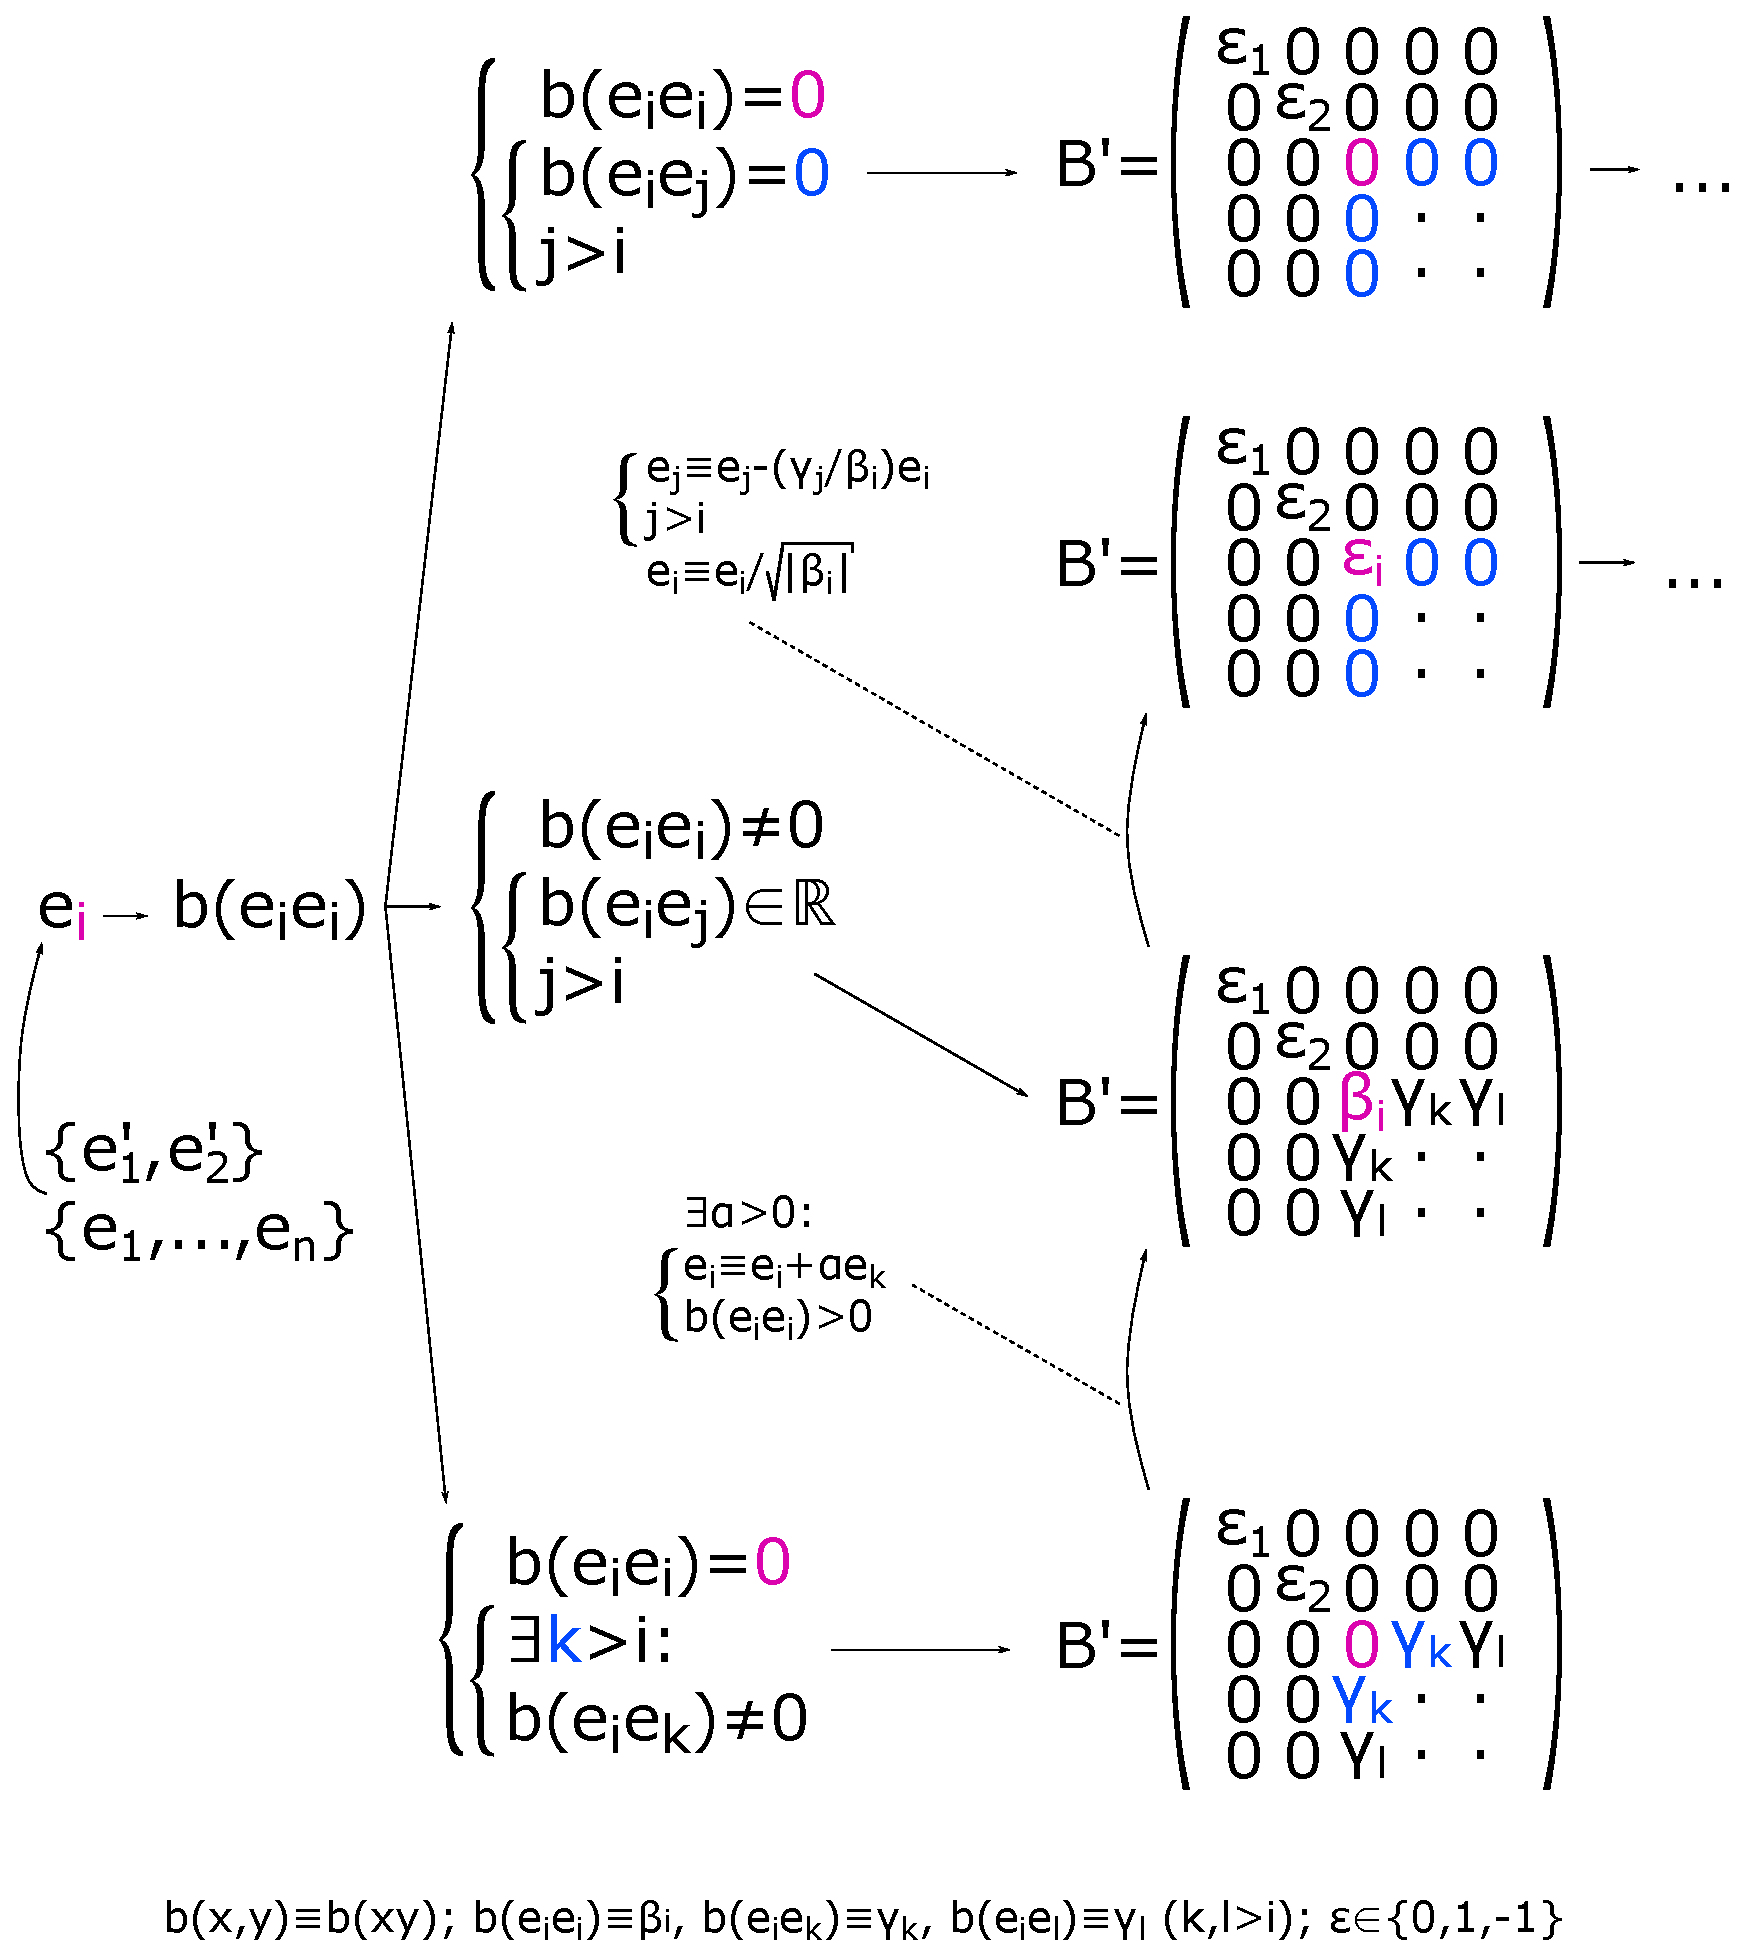
\includegraphics[width=0.85\columnwidth]{sym-bili-diag-scheme}
  
    \caption{Возможные случаи при рассмотрении очередного вектора $\bds e_i$ ``старого'' базиса при добавлении его под тем же номером в ``новый'' базис (в котором матрица билинейной функции будет канонической). Базис $e'$ строится постепенно: на каждой итерации добавляется новый вектор, а к матрице $B'$ при этом добавляется новый ``слой'', новый ``угол'' из строчки и столбца с вершиной на главной диагонали (вершина ``угла'' принимает значения $\{0, \pm 1\}$, а остальные элементы ``угла'' нули). Поэтому если все $b(\bds e_i, \bds e_j) \hm= 0$, $j \hm> i$, то ничего вообще делать не нужно, кроме, возможно, ``нормировки'' вектора $\bds e_i$. Если же $b(\bds e_i, \bds e_i) \hm{\not=} 0$ и при этом какие-то из $b(\bds e_i, \bds e_j)$, $j \hm> i$ тоже не нули, то надо ``править'' эти векторы $\bds e_j$, вычитая с нужным коэффициентом вектор $\bds e_i$, то есть $\bds e_j \hm\equiv \bds e_j \hm- b(\bds e_i, \bds e_j) \hm/ b(\bds e_i, \bds e_i) \hm\cdot \bds e_i$ (после этого будет $b(\bds e_i, \bds e_j) \hm= 0$). А если оказалось, что $b(\bds e_i, \bds e_i) \hm= 0$ и при этом хоть какой-то $b(\bds e_i, \bds e_k)$, $k \hm> i$ не ноль, то ``правим'' $\bds e_i$: надо прибавить к нему с некоторым коэффициентом $\alpha$ вектор $\bds e_k$, так чтобы $b(\bds e_i, \bds e_i)$ стало не нулём. То есть замена $\bds e_i \hm\equiv \bds e_i \hm+ \alpha \bds e_k$, и тогда $b(\bds e_i, \bds e_i) \hm= 0 \hm+ \alpha^2 b(\bds e_k, \bds e_k) \hm+ 2 \alpha b(\bds e_i, \bds e_k) \hm{\not=} 0$ при некотором~$\alpha$.}
    \label{fig:sym-bili-diag-scheme}
  \end{figure}
  
  Покажем ``по-честному'', как меняется матрица билинейной формы при смене базиса.
  И далее сформулируем утверждение о возможности приведения этой матрицы к диагональному виду.

  Пусть в базисе $e$ матрица билинейной функции $b(\cdot, \cdot)$ есть~$B$.
  Пусть ``новый'' базис $e'$ связан со ``старым'' матрицей перехода~$S$, то есть $e' \hm= eS$.
  Какой будет матрица~$B'$ билинейной функции в ``новом'' базисе?
  Значение билинейной функции на произвольной паре векторов не зависит от базиса:
  \[
    (x')^T B' y' = b(\bds x, \bds y) = x^T B y
  \]

  Пользуясь связью $x \hm= Sx'$ между координатными столбцами одного и того же вектора в разных базисах, можем преобразовать соотношение:
  \begin{equation}\label{eq:matrices-in-the-middle}
  \begin{split}
    \underline{(x')^T B' y'} = b(\bds x, \bds y) &= x^T B y\\
    &= (Sx')^T B (Sy') = \underline{(x')^T (S^T B S) y'}
  \end{split}
  \end{equation}
  
  
  % TODO: kostyl to leave the figure with big caption on separate page (move text to new page)
  \newpage
  
  \hfill \vphantom{.}
  
  \newpage
  
  
  И это верно для \emph{любой} пары $x', y' \hm\in \RR$.
  Поэтому можно утверждать, что будут равны матрицы ``посередине'':
  \begin{equation}\label{eq:matrix-change}
    \boxed{B' = S^T B S}
  \end{equation}
  (Подставляя $x' \hm= y' \hm= (1, 0, \ldots, 0)^T$ в~(\ref{eq:matrices-in-the-middle}), получаем равенство элементов матриц на позиции ``$1,1$''.
  Подставляя $x' \hm= (1, 0, 0, \ldots, 0)$ и $y' \hm= (0, 1, 0, \ldots, 0)$, получаем равенство элементов на позиции ``$1,2$''.
  И так далее.)

  \begin{theorem}
    Пусть $b(\cdot, \cdot)$ есть симметричная билинейная функция.
    Тогда найдётся базис~$e'$, в котором матрица~$B'$ билинейной функции будет диагональной
    \[
      B' = \diag(\eps_1, \ldots, \eps_n),\quad \eps_i \in \RR
    \]
    
    Более того, найдётся базис $e''$, в котором матрица~$B''$ билинейной функции будет диагональной, причём на диагонали будут обязательно только числа $\{0, 1, -1\}$:
    \begin{equation}\label{eq:canonical-matrix}
      B'' = \diag(\eps_1, \ldots, \eps_n),\quad \eps_i \in \{0, \pm 1\}
    \end{equation}
  \end{theorem}
  
  Также можно привести ``матричный аналог'' утверждения.
  
  \begin{theorem}
    Пусть $B \hm\in \RR^{n \times n}$ есть симметричная матрица.
    Тогда найдётся невырожденная квадратная матрица $S \hm\in \RR^{n \times n}$, такая что матрица $S^T B S$ будет диагональной:
    \[
      B' = S^T B S = \diag(\eps_1, \ldots, \eps_n),\quad \eps_i \in \RR
    \]
    
    Более того, найдётся невырожденная квадратная матрица $S \hm\in \RR^{n \times n}$, такая что матрица $S^T B S$ будет диагональной, причём на диагонали будут только числа $\{0, 1, -1\}$:
    \[
      B'' = S^T B S = \diag(\eps_1, \ldots, \eps_n),\quad \eps_i \in \{0, \pm 1\}
    \]
  \end{theorem}
  
  
  \subsection{Канонический вид k(x)}
  
  Если в данном базисе $e$ матрица квадратичной функции~$k(\bds x)$ имеет вид~(\ref{eq:canonical-matrix}), то есть диагональная с числами $\{0, \pm 1\}$ на диагонали, то говорят, что форма в базисе~$e$ имеет \emph{канонический вид}.
  
  \begin{example}
    Форма $k(\bds x)$ в каноническом виде может, например, иметь матрицу:
    \[
      B = \begin{pmatrix}
        1 & 0  & 0\\
        0 & -1 & 0\\
        0 & 0  & 1\\
      \end{pmatrix}
    \]
    
    Тогда формула для нахождения $k(\bds x)$:
    \[
      k(\bds x) = x_1^2 - x_2^2 + x_3^2
    \]
  \end{example}
  
  Количество ненулевых элементов на диагонали матрицы~$B'$ формы~$k(\cdot)$ в каноническом виде, очевидно, определяет ранг~$B'$.
  А что можно сказать о ранге матрицы~$B$ формы~$k(\cdot)$ в произвольном базисе?
  Оказывается, что $\Rg B \hm= \Rg B'$:
  \[
    B' = S^T B S \Rightarrow \Rg B' = \Rg (S^T B S) = \Rg (S^T B) = \Rg B
  \]
  
  Канонический вид формы зависит от базиса.
  Например, одна и та же форма может иметь канонический вид $k(\bds x) \hm= x_1^2 - x_2^2$ с матрицей $B' \hm= \left(\begin{smallmatrix} 1 & 0 \\ 0 & -1 \end{smallmatrix}\right)$ в одном базисе и иметь вид $k(\bds x) \hm= -x_1^2 + x_2^2$ с матрицей $B'' \hm= \left(\begin{smallmatrix} -1 & 0 \\ 0 & 1 \end{smallmatrix}\right)$ в другом базисе.
  Но зависит ли ранг матрицы формы в каноническом виде от способа приведения формы к этому каноническому виду?
  То есть обязательно ли $\Rg B' \hm= \Rg B''$, если $B'$ и $B''$ определяют канонический вид одной и той же формы в разных базисах?
  Очевидно, да, ведь по уже доказанному
  \[
    \Rg B' = \Rg B = \Rg B''
  \]
  где $B$~---~матрица формы в произвольном ``начальном'' базисе.
  Независимость ранга матрицы от способа приведения формы к каноническому виду можно бы было показать и по-другому, от противного.
  
  \begin{example}
    Так, допустим, что у одной формы $k(\cdot)$ получилось в разных базисах получить такие матрицы:
    \[
      B' = \begin{pmatrix}
        1 & 0 & 0\\
        0 & 1 & 0\\
        0 & 0 & -1
      \end{pmatrix},\quad B'' = \begin{pmatrix}
        1 & 0 & 0\\
        0 & 0 & 0\\
        0 & 0 & 0
      \end{pmatrix}
    \]
    
    Почему такого не может быть?
    Потому что для формы с матрицей~$B''$ можно привести двумерное подпространство
    \[
      U'' = \left\{
        \begin{pmatrix}
          0\\
          x_2''\\
          x_3''
        \end{pmatrix}\ \Biggm|\ x_2'', x_3'' \in \RR
      \right\}
    \]
    на котором форма будет нулевой:
    \[
      \bds x \in U'' \to k(\bds x) = x^T B'' x = 0
    \]
    
    Однако для формы с матрицей~$B'$ подобного двумерного подпространства уже не найти.
    ...Это очевидно.
    ...Очевидно ли?
    Пожалуй, не совсем...
    
    Несложно найти два \emph{одномерных} подпространства
    \[
      U_1' = \left\{
        \begin{pmatrix}
          x_1'\\
          0\\
          x_3'
        \end{pmatrix}\ \Biggm|\ x_1' = x_3' \in \RR
      \right\},\quad U_2' = \left\{
        \begin{pmatrix}
          0\\
          x_2'\\
          x_3'
        \end{pmatrix}\ \Biggm|\ x_2' = x_3' \in \RR
      \right\}
    \]
    на которых $k(\bds x) \hm= x^T B' x \hm= 0$.
    Однако сумма $U_1' \hm+ U_2'$ не будет давать двумерное подпространство, для векторов которого $k(\bds x) \hm= 0$.
    
    Проще получить противоречие (и в более общем случае, а не только в рассмотренном примере), возможно, было бы, если бы рассматривались не подпространства, где форма \emph{обязательно нулевая}, а где она \emph{может быть ненулевая}.
    Так, для формы с матрицей~$B''$ максимальное по размерности подпространство с таким свойством будет одномерным: натянутым на вектор $u'' \hm= (1, 0, 0)^T$.
    А для формы с матрицей~$B'$ оно будет трёхмерным.
    Имеется в виду, что можно привести три линейно независимых вектора: $u' \hm= (1, 0, 0)^T$, $v' \hm= (0, 1, 0)^T$ и $w' \hm= (0, 0, 1)^T$~---~таких что $u^{\prime T} B' u' \hm= v^{\prime T} B' v' \hm= w^{\prime T} B' w' \hm= 0$.
  \end{example}
  
  Итого, ранг матрицы квадратичной формы сохраняется при переходе к новому базису.
  И в любом каноническом виде одной и той же квадратичной формы число ненулевых значений ($\pm 1$) на диагонали будет одинаковым.
  Но может ли получиться так, что будет разным, например, количество значений $+1$?
  
  \begin{example}
    Допустим, что у одной формы $k(\cdot)$ получилось в разных базисах получить такие матрицы:
    \[
      B' = \begin{pmatrix}
        1 & 0 & 0\\
        0 & 0 & 0\\
        0 & 0 & -1
      \end{pmatrix},\quad B'' = \begin{pmatrix}
        1 & 0 & 0\\
        0 & 1 & 0\\
        0 & 0 & 0
      \end{pmatrix}
    \]
    
    Имея матрицу~$B'$, можно указать такое \emph{максимальное по размерности подпространство, на котором форма положительно определена}:
    \[
      L'_{+} = \left\{
        \begin{pmatrix}
          x_1'\\
          0\\
          0
        \end{pmatrix}\ \Biggm|\ x_1' \in \RR
      \right\},\quad k(\bds x) = x^T B' x > 0,\ \forall \bds x \in L'_{+}, \bds x \not= \bds 0
    \]
    
    А в том базисе, в котором дана~$B''$, это будет двумерное подпростнанство:
    \[
      L''_{+} = \left\{
        \begin{pmatrix}
          x_1''\\
          x_2''\\
          0
        \end{pmatrix}\ \Biggm|\ x_1'', x_2'' \in \RR
      \right\},\quad k(\bds x) = x^T B'' x > 0,\ \forall \bds x \in L''_{+}, \bds x \not= \bds 0
    \]
    
    Получается, $L'_{+} \hm{\not=} L''_{+}$, так как $\dim L'_{+} \hm{\not=} \dim L''_{+}$.
    Однако само понятие \emph{максимального по размерности подпространства, на котором форма положительно определена} не зависит от базиса, а характеризует лишь саму квадратичную форму.
    Пришли к противоречию.
  \end{example}
  
  Понятия $L^{+}$ и $L^{-}$ (подпространства максимальной размерности, на которых форма определена соответственно положительно и отрицательно) позволяют аналогичным образом показать неизменность количества значений $+1$ и $-1$ на диагонали в каноническом виде для произвольной квадратичной формы.
  Поэтому можно ввести понятия: \emph{положительный индекс} квадратичной формы~$p$ и \emph{отрицательный индекс} квадратичной формы~$q$~---~как числа единичек и минус единичек в каноническом виде квадратичной формы.
  Ранг матрицы формы, очевидно, оказывается равным сумме $p \hm+ q$.
  \emph{Сигнатурой}~$\sigma$ квадратичной формы называется разность $p \hm- q$.
  
  \begin{theorem}
    Ранг, положительный и отрицательный индексы, сигнатура не зависят от базиса, в котором форма приведена к каноническому виду (и потому являются характеристиками не столько матрицы формы в конкретном базисе, сколько самой формы).
  \end{theorem}
  
  
  \subsection{Положительная определённость k(x)}
  
  На нескольких примерах разберём некоторые особенности положительно и отрицательно определённых форм, которые следуют из вида их матриц в каноническом виде.
  
  \begin{example}
    Пусть $B$ есть матрица некоторой \emph{положительно определённой} квадратичной формы~$k(\cdot)$ в трёхмерном пространстве:
    \[
      B = \begin{pmatrix}
        b_{11} & b_{12} & b_{13}\\
        b_{21} & b_{22} & b_{23}\\
        b_{31} & b_{32} & b_{33}
      \end{pmatrix},\ B = B^T
    \]
    
    Раз форма~$k(\cdot)$ положительно определена, то в каноническом виде у неё обязательно будет матрица:
    \[
      B' = \begin{pmatrix}
        1 & 0 & 0\\
        0 & 1 & 0\\
        0 & 0 & 1
      \end{pmatrix}
    \]
    
    И соответствующая формула $k(\bds x)$ от координат вектора:
    \[
      k(\bds x) = x_1^{\prime 2} + x_2^{\prime 2} + x_3^{\prime 2}
    \]
    
    Что можно заметить ``интересного'' про матрицу~$B'$?
    Она полного ранга.
    А ранг матрицы формы сохраняется при смене базиса.
    Таким образом, \emph{матрица положительно определённой квадратичной формы полного ранга}.
    
    Что-нибудь ещё ``интересное''?
    Не сложно заметить, что $\det B' \hm= 1$.
    А что можно сказать про определитель исходной~$B$?
    как он связан (и связан ли вообще как-нибудь) с определителем~$B'$?
    \[
      \det B' = \det (S^T B S) = \det S^T \det B \det S = (\det S)^2 \det B
    \]
    
    То есть из того, что $\det B' \hm= 1 \hm> 0$ следует, что и $\det B \hm> 0$.
    Таком образом, \emph{определитель матрицы положительно определённой квадратичной формы больше нуля}.
    
    Посмотрим ещё раз внимательно на матрицу формы~$B'$ и заметим, что...
    больше нуля не только $\det B'$~---~положительны определители всех квадратных подматриц, расположенных в левом верхнем углу!
    (Такие определители называются \emph{главными минорами} и обычно обозначаются как $\Delta_i$, где $i \hm\geq 1$ есть порядок минора.)
    То есть
    \[
      \Delta_1' = 1 > 0,
      \quad \Delta_2' = \begin{vmatrix}
        1 & 0\\
        0 & 1
      \end{vmatrix} = 1 > 0,
      \quad \Delta_3' = \det B' = 1 > 0
    \]
    
    Можно ли утверждать то же самое и про матрицу~$B$?
    Ведь про определитель всей матрицы получилось показать, что он тоже больше нуля...
    Посмотрим:
    \[
      \Delta_1 = b_{11} = k(\bds e_1) > 0
    \]
    так как форма по условию положительно определена.
    А какого знака будет второй главный минор?
    \[
      \Delta_2 = \begin{vmatrix}
        b_{11} & b_{12}\\
        b_{21} & b_{22}
      \end{vmatrix}
    \]
    
    Рассмотрим двумерное подпространство векторов:
    \[
      U = \left\{
        \begin{pmatrix}
          x_1\\
          x_2\\
          0
        \end{pmatrix}\ \Biggm|\ x_1, x_2 \in \RR
      \right\}
    \]
    
    Раз форма~$k(\cdot)$ положительно определена на всём пространстве, то она положительно определена и на подпространстве~$U$, то есть $k(\bds x) \hm> 0$ для всех ненулевых $\bds x \hm\in U$.
    Подставим координаты произвольного вектора из~$U$ в формулу $k(\cdot)$ и немного преобразуем, или ``перепишем'', не меняя сути:
    \[
      k(\bds x)
      = (x_1, x_2, 0)^T \begin{pmatrix}
        b_{11} & b_{12} & b_{13}\\
        b_{21} & b_{22} & b_{23}\\
        b_{31} & b_{32} & b_{33}
      \end{pmatrix} \begin{pmatrix}
        x_1\\
        x_2\\
        0
      \end{pmatrix}
      = (x_1, x_2)^T \begin{pmatrix}
        b_{11} & b_{12}\\
        b_{21} & b_{22}
      \end{pmatrix} \begin{pmatrix}
        x_1\\
        x_2
      \end{pmatrix}
    \]
    
    Иными словами, положительная определённость формы вкупе с ``упрощённой формулой'' вычисления $k(\cdot)$ для векторов  из $U$ выливаются в:
    \[
      (x_1, x_2)^T \begin{pmatrix}
        b_{11} & b_{12}\\
        b_{21} & b_{22}
      \end{pmatrix} \begin{pmatrix}
        x_1\\
        x_2
      \end{pmatrix} > 0\quad \forall (x_1, x_2)^T \not= 0
    \]
    
    А это фактически означает, что положительно определена некоторая форма с матрицей $\left(\begin{smallmatrix}
      b_{11} & b_{12}\\
      b_{21} & b_{22}
    \end{smallmatrix}\right)$!
    Но определитель матрицы положительно определённой формы обязательно положителен!
    То есть и второй главный минор~$\Delta_2$ матрицы~$B$ больше нуля.
    
    Таким образом, \emph{все главные миноры матрицы положительно определённой квадратичной формы больше нуля}.
  \end{example}
  
  Все приведённые выводы про матрицу положительно определённой квадратичной формы из примера, очевидно, будут верны и для положительно определённой формы произвольного порядка.
  Однако последнее наблюдение, про главные миноры, не такое простое (ещё более непростое), как пока могло показаться.
  
  \begin{example}
    Пусть $B$ есть матрица \emph{некоторой} квадратичной формы~$k(\cdot)$ в трёхмерном пространстве:
    \[
      B = \begin{pmatrix}
        b_{11} & b_{12} & b_{13}\\
        b_{21} & b_{22} & b_{23}\\
        b_{31} & b_{32} & b_{33}
      \end{pmatrix},\ B = B^T
    \]
    
    Известно, что главные миноры матрицы положительны.
    \emph{Следует ли из этого, что форма положительно определена}?
    Иными словами, обязательно ли матрица~$B'$ формы в каноническом виде будет иметь вид:
    \[
      \begin{pmatrix}
        1 & 0 & 0\\
        0 & 1 & 0\\
        0 & 0 & 1
      \end{pmatrix}
    \]

    Начнём с того, что посмотрим на определитель $\det B'$:
    \[
      \det B' = \det (S^T B S) = (\det S)^2 \det B
    \]
    раньше эта формула уже использовалась, но тогда было ``в другую сторону''.
    Теперь же важно, что знак $\det B'$ такой же, как у $\det B$, то есть тоже больше нуля, так как $\det B \hm= \Delta_3 \hm> 0$ по условию.
    Таким образом, у матрицы $B'$ формы в каноническом виде точно полный ранг, то есть на диагонали нет нулей:
    \[
      B' = \begin{pmatrix}
        \eps_1 & 0      & 0\\
        0      & \eps_2 & 0\\
        0      & 0      & \eps_3
      \end{pmatrix},\quad \eps_i \not= 0
    \]
    
    Далее, так как
    \[
      \Delta_2 = \begin{vmatrix}
        b_{11} & b_{12}\\
        b_{21} & b_{22}
      \end{vmatrix} > 0
    \]
    то у некоторой формы $\widetilde{k\hphantom{\,}} (\cdot)$ с матрицей $\left(  % TODO: normal way for normal size tilde for k(*)
      \begin{smallmatrix}
        b_{11} & b_{12}\\
        b_{21} & b_{22}
      \end{smallmatrix}
    \right)$ в каноническом виде будет матрица $\tilde B' \hm= \diag(\tilde \eps_1, \tilde \eps_2)$, \emph{определитель которой тоже больше нуля}.
    И так как \emph{матрица~$B$ исходной формы невырождена}, то \emph{можно} организовать процесс приведения к каноническому виду следующим образом:
    \[
      B = \begin{pmatrix}
        b_{11} & b_{12} & b_{13}\\
        b_{21} & b_{22} & b_{23}\\
        b_{31} & b_{32} & b_{33}
      \end{pmatrix} \sim \begin{pmatrix}
        \tilde \eps_1 & 0             & b_{13}\\
        0             & \tilde \eps_2 & b_{23}\\
        b_{31} & b_{32} & b_{33}
      \end{pmatrix} \sim \begin{pmatrix}
        \tilde \eps_1 & 0             & 0\\
        0             & \tilde \eps_2 & 0\\
        0             & 0             & \eps_3
      \end{pmatrix}
    \]
    то есть сначала как бы приводим к каноническому виду подматрицу второго порядка в верхнем левом углу, которая есть матрица положительно определённой формы $\widetilde{k\hphantom{\,}} (\cdot)$, а потом уже ``доделываем'' последние столбец и строчку.
    Итого, получается, что
    \[
      \det B' = \underbrace{\overbrace{\det \tilde B'}^{> 0} \cdot \eps_3}_{> 0}
    \]
    но тогда обязательно $\eps_3 \hm> 0$, то есть $\boxed{\eps_3 \hm= 1}$!
    (Так как канонический вид.)
    
    То есть узнали чуть больше про $B'$~---~теперь понятно, что
    \[
      B' = \begin{pmatrix}
        \eps_1 & 0      & 0\\
        0      & \eps_2 & 0\\
        0      & 0      & 1
      \end{pmatrix},\quad \eps_i \not= 0
    \]
    
    Аналогично можно показать, что $\eps_2 \hm= 1$, а потом и $\eps_1 \hm= 1$.
    В итоге у матрицы~$B'$ формы в каноническом виде только единицы на диагонали~---~а это и есть критерий положительной определённости формы.
  \end{example}
  
  С некоторыми, возможно, дополнительными ``аккуратностями'' рассуждения из примера применимы и к форме с матрицей произвольного порядка с тем свойством, что все её главные миноры больше нуля.
  
  Наблюдения из нескольких рассмотренных выше примеров иллюстрируют следующее утверждение.
  
  \begin{theorem}[Критерий Сильвестра]
    Для положительной определённости квадратичной формы $k(\cdot)$ с матрицей $B \hm\in \RR^{n \times n}$ в некотором базисе необходимо и достаточно, чтобы все главные миноры этой матрицы $\Delta_i$ $(i \hm= 1, \ldots, n)$ были больше нуля.
  \end{theorem}
  
  А что же с отрицательной определённостью?
  С некоторыми незначительными отличиями рассуждения, приведённые в примерах с положительно определённой формой, ``работают''  и в случае с отрицательно определённой формой.
  Главное, что меняется~---~это то, что знак определителя матрицы формы (очевидно~---~в каноническом, а далее можно показать, что и вообще в любом виде) \emph{зависит от порядка матрицы}, то есть чередуется, то ``плюс'', то ``минус''.
  
  \begin{theorem}[``Критерий Сильвестра 2'']
    Для отрицательной определённости квадратичной формы $k(\cdot)$ с матрицей $B \hm\in \RR^{n \times n}$ в некотором базисе необходимо и достаточно, чтобы знаки всех главных миноров этой матрицы $\Delta_i$ $(i \hm= 1, \ldots, n)$ чередовались как $(-1)^i$, то есть
    \[
      \underline{\Delta_1 \hm< 0} \leftrightarrow -1 \hm < 0,\quad \underline{\Delta_2 \hm> 0} \leftrightarrow (-1) \cdot (-1) \hm> 0,\quad \ldots
    \]
    % Looks good, but understanding questionable
    %\[
      %\left\{
        %\begin{aligned}
          %&\Delta_i < 0,\quad i \equiv 1 \pmod 2\\
          %&\Delta_i > 0,\quad i \equiv 0 \pmod 2\\
        %\end{aligned}
      %\right.
    %\]
  \end{theorem}


  \section{Задачи}
  
  \subsection{по мотивам \# 32.8(2) + 32.9(2)}
  
  Привести данную квадратичную форму
  \[
    k(\bds x) = x_1^2 - x_1 x_2 - 2 x_1 x_3 + \frac{x_2^2}{4} + x_3^2
  \]
  к каноническому виду с помощью метода Лагранжа или элементарных преобразований (столбцов и строк!) её матрицы.
  Найти ранг, положительный и отрицательный индексы инерции и сигнатуру этой формы.

  Выяснить, является ли форма положительно или отрицательно определённой или полуопределённой.
  
  \begin{solution}
    {}\hfill\par
    
    \emph{Способ 1: Метод Лагранжа (выделения квадратов)}.

    В формуле $k(\bds x)$ есть член $x_1^2$, а также члены с $x_1$ в первой степени.
    Поэтому приведение к каноническому виду можно начать с того, чтоб \emph{собрать вместе все члены с $x_1$, дополнить, если надо, до квадрата, и сделать замену, выделив квадрат} (так, чтобы члены с $x_1$ ``ушли'', а вместо этого появился бы только квадрат новой переменной):
    \[
      k(\bds x) = \left(x_1^2 - x_1 x_2 - 2 x_1 x_3 + \underline{\left(\frac{x_2}{2}\right)^2 + x_3^2 + 2 \cdot \frac{x_2}{2} \cdot x_3}\right) - \underline{\left(\frac{x_2}{2}\right)^2 - x_3^2 - 2 \cdot \frac{x_2}{2} \cdot x_3} + \frac{x_2^2}{4} + x_3^2
    \]
    \[
      k(\bds x) = \left(x_1 - \frac{x_2}{2} - x_3\right)^2 - x_2 x_3
    \]
    
    Замена:
    \begin{equation}\label{eq:p1-var-change1}
      \left\{
        \begin{aligned}
          &x_1' = x_1 - \frac{x_2}{2} - x_3\\
          &x_2' = x_2\\
          &x_3' = x_3
        \end{aligned}
      \right.
    \end{equation}
    
    В результате формула для квадратичной функции примет вид:
    \[
      k(\bds x) = x_1^{\prime 2} - x_2' x_3'
    \]
    
    При приведении формы к диагональному (или каноническому) виду методом Лагранжа может возникнуть ситуация, когда квадрат сразу выделить и нельзя.
    Как в формуле выше: есть только смешанное произведение~$x_2' x_3'$, но ни $x_2^{\prime 2}$, ни $x_3^{\prime 2}$ нет.
    В таком случае можно сделать следующую замену (``трюк''):
    \begin{equation}\label{eq:p1-var-change2}
      \left\{
        \begin{aligned}
          &x_1' = x_1''\\
          &x_2' = x_2'' - x_3''\\
          &x_3' = x_2'' + x_3''
        \end{aligned}
      \right.
    \end{equation}
    
    В результате вместо $x_2' x_3'$ появится разность квадратов, и ``стандартный'' процесс выделения квадратов и замен переменных можно будет продолжить:
    \[
      k(\bds x) = x_1^{\dprime 2} - (x_2'' - x_3'') (x_2'' + x_3'')
    \]
    \begin{equation}\label{eq:p1-canonical}
      k(\bds x) = x_1^{\dprime 2} - x_2^{\dprime 2} + x_3^{\dprime 2}
    \end{equation}
    
    Привели форму к каноническому виду.
    Теперь, по-хорошему, надо ещё привести соответствующую замену координат (переход от ``старого'' исходного базиса к ``новому'', где канонический вид).
    Из первой замены~(\ref{eq:p1-var-change1}) получаем:
    \[
      \left\{
        \begin{aligned}
          &x_1 = x_1' + \frac{x_2'}{2} + x_3'\\
          &x_2 = x_2'\\
          &x_3 = x_3'
        \end{aligned}
      \right. \quad\leftrightarrow\quad x = S_1 x',\quad S_1 = \begin{pmatrix}
        1 & 1/2 & 1\\
        0 & 1 & 0\\
        0 & 0 & 1
      \end{pmatrix}
    \]
    где $S_1$~---~матрица, задающая переход от базиса~$e$ к базису $e'$ (в котором координаты с одним ``штрихом'').
    Далее, вторая замена~(\ref{eq:p1-var-change2}):
    \[
      \left\{
        \begin{aligned}
          &x_1' = x_1''\\
          &x_2' = x_2'' - x_3''\\
          &x_3' = x_2'' + x_3''
        \end{aligned}
      \right. \quad\leftrightarrow\quad x' = S_2 x'',\quad S_2 = \begin{pmatrix}
        1 & 0 & 0\\
        0 & 1 & -1\\
        0 & 1 & 1
      \end{pmatrix}
    \]
    где $S_2$~---~матрица перехода от базиса~$e'$ к базису $e''$ (в котором как раз имеем канонический вид формы~(\ref{eq:p1-canonical})).
    
    Итоговая (комбинированная) замена:
    \[
      \left\{
        \begin{aligned}
          &x_1 = x_1'' + \frac{3 x_2''}{2} + \frac{x_3''}{2}\\
          &x_2 = x_2'' - x_3''\\
          &x_3 = x_2'' + x_3'
        \end{aligned}
      \right. \quad\leftrightarrow\quad x = S x'',\quad S = \begin{pmatrix}
        1 & 3/2 & 1/2\\
        0 & 1 & -1\\
        0 & 1 & 1
      \end{pmatrix}
    \]
    
    Можно проверить, что $S \hm= S_1 S_2$:
    \[
      S_1 S_2 = \begin{pmatrix}
        1 & 1/2 & 1\\
        0 & 1 & 0\\
        0 & 0 & 1
      \end{pmatrix} \begin{pmatrix}
        1 & 0 & 0\\
        0 & 1 & -1\\
        0 & 1 & 1
      \end{pmatrix} = \begin{pmatrix}
        1 & 3/2 & 1/2\\
        0 & 1 & -1\\
        0 & 1 & 1
      \end{pmatrix} = S
    \]
    
    \bigskip
    
    \emph{Способ 2: Элементарные преобразования матрицы (столбцов и строк)}.
    
    При смене базиса матрица формы меняется по правилу~(\ref{eq:matrix-change}):
    \[
      B' = S^T B S
    \]
    
    Матрица $S$ невырожденная, поэтому может быть представлена как произведение матриц, задающих, например, элементарные преобразования столбцов: $S \hm= S_1 \hm\cdot \ldots \hm\cdot S_N$.
    Если подставить это в формулу выше:
    \[
      B' = S_N^T \cdot \ldots \cdot S_1^T \cdot B \cdot S_1 \cdot \ldots \cdot S_N
    \]
    Получается, чтобы получить $B'$, надо провести над $B$ серию преобразований: столбцов (умножение на $S_i$ справа) и строк (умножение на $S_i^T$ слева), причём после преобразования столбцов должно сразу идти аналогичное преобразование строк (например, первая пара преобразований: $S_1^T B S_1$).
    
    С помощью способа, похожего на тот, с помощью которого искали обратную матрицу, можно одновременно найти и диагональную (каноническую) матрицу~$B'$ формы, и матрицу перехода~$S$ к соответствующему базису: надо ``приписать'', например, справа к исходной матрице единичную, и выполнять над ней те же самые элементарные преобразования, но \textbf{только элементарные преобразования столбцов}:
    \[
      (B \mid E) \to (S_1^T B S_1 \mid S_1) \to \ldots \to (S_N^T \ldots S_1^T B S_1 \ldots S_N \mid \underbrace{S_1 \ldots S_N}_{S})
    \]
    
    Возвращаясь к форме из задачи, её матрица:
    \[
      B = \begin{pmatrix}
        1    & -1/2 & -1\\
        -1/2 & 1/4  & 0\\
        -1   & 0    & 1
      \end{pmatrix}
    \]
    
    Получим из неё диагональную:
    \begin{equation}
    \begin{split}
      \left(
        \begin{matrix}
          1    & -1/2 & -1\\
          -1/2 & 1/4  & 0\\
          -1   & 0    & 1
        \end{matrix}
        \BigMiddleThree
        \begin{matrix}
          1 & 0 & 0\\
          0 & 1 & 0\\
          0 & 0 & 1
        \end{matrix}
      \right)
      \sim \left(
        \begin{matrix}
          1 & 0    & 0\\
          0 & 0    & -1/2\\
          0 & -1/2 & 0
        \end{matrix}
        \BigMiddleThree
        \begin{matrix}
          1 & 1/2 & 1\\
          0 & 1   & 0\\
          0 & 0   & 1
        \end{matrix}
      \right)
      \sim \left(
        \begin{matrix}
          1 & 0  & 0\\
          0 & -1 & 0\\
          0 & 0  & 1
        \end{matrix}
        \BigMiddleThree
        \begin{matrix}
          1 & 3/2 & 1/2\\
          0 & 1   & -1\\
          0 & 1   & 1
        \end{matrix}
      \right)
    \end{split}
    \end{equation}
    где первый переход~---~это результат преобразования ``ко второму столбцу прибавить половину первого, к третьему прибавить первый'' (и то же самое со строками~---~но только для матрицы ``слева''), а второй~---~это ``ко второму столбцу прибавить третий, а из третьего вычесть второй'' (и потом так же со строками).
    
    Итого, матрица формы $B'$ в каноническом виде и матрица перехода~$S$ к соответствующему базису\footnote{
    ...Внимательный читатель мог заметить, что стадии изменения матрицы в процессе элементарных преобразований в точности соответствуют заменам, совершённым в процессе диагонализации методом Лагранжа!
    Однако стоит считать это лишь ``случайностью''~---~вообще могло бы получиться и по-другому.}:
    \[
      B' = \begin{pmatrix}
        1 & 0  & 0\\
        0 & -1 & 0\\
        0 & 0  & 1
      \end{pmatrix},\quad S = \begin{pmatrix}
        1 & 3/2 & 1/2\\
        0 & 1   & -1\\
        0 & 1   & 1
      \end{pmatrix}
    \]
    
    \bigskip
    
    Имея форму в каноническом виде~(\ref{eq:p1-canonical}):
    \[
      k(\bds x) = x_1^{\dprime 2} - x_2^{\dprime 2} + x_3^{\dprime 2}
    \]
    не сложно ответить на вопрос о знакоопределённости формы.
    Она будет знакопеременной.
    Потому что, например, при $u'' \hm= (1, 0, 0)^T$ имеем $k(u'') \hm> 0$, а при $v'' \hm= (0, 1, 0)^T$ получается $k(v'') \hm< 0$.
  \end{solution}
\end{document}
